\chapter{RUST}
\textbf{Rust} is a general purpose, system programming language
with a focus on safety, especially \textbf{safe concurrency},
supporting both \textit{functional} and \textit{imperative} paradigms.
Its main goal is to \textit{ensure \underline{safety} without penalizing \underline{efficiency}}.\\
\texttt{C/C++} provide more control but less safety, while \texttt{Python/Haskell} provide less control but more safety.
\textbf{Rust} aims to get the best of both worlds, providing both \textbf{control} and \textbf{safety}.

Despite its syntax resemblance to C/C++, in a deeper sense Rust is closer to the ML family languages;
in fact almost every part of a function body is an expression, include \texttt{if-then-else} constructs, which returns a value.

\section{Statically enforcing memory safety}
Rust, similarly to C, compiles to \textbf{object code} for bare-metal performance,
but it supports \textbf{memory safety}:
programs can \ul{\textit{dereference} only previously allocated pointers that have
not been freed}, and \ul{\textit{out-of-bound} array accesses not allowed};
besides, the \textbf{overhead} introduced is very low, since it's the \textit{compiler} which checks that memory safety rules are followed,
and there's \textit{\underline{no} garbage collection}, so zero-cost abstraction in managing memory.\\
{This is achieved through and \textbf{advanced type system} and three key concepts to prevent memory corruption:\ns
\begin{enumerate}
   \item \textbf{Ownership}
   \item \textbf{Borrowing}
   \item \textbf{Lifetime}
\end{enumerate}}

Again, Rust is designed to be \ul{\textbf{memory safe} even in the presence
of \textbf{concurrency}}, and guarantees the following properties \textbf{statically}, meaning that
if the program \textit{compiles} it will \textit{never manifest a violation} of these properties: 
\begin{itemize}
   \item No \texttt{null} pointers\\
   $\longrightarrow$ accessing a variable which does not hold a value
   \item No dangling pointers\\
   $\longrightarrow$ Pointers to invalid memory location
   \begin{itemize}
      \item Pointers to explicitly deallocated objects;
      \item Pointers to locations beyond the end of an array;
      \item Pointers to objects allocated on the stack;
   \end{itemize}
   \item No double frees\\
   $\longrightarrow$ A memory location in the heap is reclaimed twice
   \item No data races\\
   $\longrightarrow$ unpredictable results in concurrent computations
   \item No iterator invalidation
\end{itemize}

\section{\texttt{null} and Primitive types in Rust}
A \texttt{null} value does \textbf{not} exist in Rust, so in some way it must address the problem of accessing a variable which does not hold a value.\\
Data values can only be initialized through a fixed set of
forms, requiring their inputs to be already initialized, and \ul{if 
any branch of code fails to assign a
value to the variable, we get a \textbf{compile time error}}.
\note{Static/global variables must be initialized at declaration
time.}
\lstset{language=Rust}
\textit{Nullable} types, are managed with a generic \lstinline|Option<T>|, playing
the role of Haskell's \texttt{Maybe} or Java's \texttt{Optional}
\begin{lstlisting}
   enum std::option::Option<T> {
      None,
      Some(T)
   }
\end{lstlisting}

\subsection{Primitive Types}
\begin{lstlisting}[caption={Rust primitive types}]
   // Numeric types:
   i8 / i16 / i32 / i64 / isize
   u8 / u16 / u32 / u64 / usize
   f32 / f64
   
   bool
   char // (4-byte unicode)
\end{lstlisting}
\begin{itemize}
\item \textbf{Type inference} for variables declarations with \lstinline|let|
\item \textbf{No overloading} for literals: type annotations to disambiguate
\item \textbf{Tuples} like in Haskell
\item \textbf{Arrays} with fixed length. 
\note{\textit{out-of-bound} access is checked at \textbf{runtime},
but it's just a single comparison, its overhead is negligible}
\end{itemize}

\section{Memory Management}
As usual, Rust uses a \textbf{stack} of activation records, and a \textbf{heap} for dynamically allocated data structures.

The user is forced to be \textit{aware of where} the data are stored: 
there is no \textbf{implicit boxing}\footnotemark.


\begin{lstlisting}
   fn main() {
      let x = 3; // 'let' allocates a variable on the stack
      let y = Box::new(3); // y is a reference to 3 on the heap
      println!("x == y is {}", x == *y); // "x == y is true"
   }

   fn main() {
      let x = 3; // 'let' allocates a variable on the stack
      let y = Box::new(3); // y is a reference to 3 on the heap
      let z = Box::new(x); // z and x are two separate things
      println!("x == *y is {}", x == *y); // "x == y is true"
      println!("z == y is {}", z == y); // "z == y is true" because Rust automatically dereferences the Box
      x = 6;
      println!("x == z == {}", *z); // evaluates to three
   }
\end{lstlisting}

To avoid the overhead of a Garbage collection mechanism and the possible subtle errors introduced a programmer to whom memory management is delegated, Rust provides \textit{deterministic management of
resources}, with very low overhead, using \textbf{RAII} (\textit{\underline{R}esource \underline{A}cquisition \underline{I}s \underline{I}nitialization}).

\subsection{Variables Immutability and \texttt{RAII}}
By \textit{default}, Rust variables are \textbf{immutable}, and their usage is statically checked by the compiler.
\lstinline|mut| is used to declare a resource as mutable.
\begin{paracol}{2}
\begin{lstlisting}[caption={ Compilation \textit{error} \xmark}]
   fn main() {
      let a: i32 = 0;
      a = a + 1;
      println!("a == {}", a);
   }
\end{lstlisting}
\switchcolumn
\begin{lstlisting}[caption={Compilation ok \cmark}]
   fn main() {
      let mut a: i32 = 0;
      a = a + 1;
      println!("a == {}", a);
   }
\end{lstlisting}
\end{paracol}
\footnotetext[1]{Act of \textit{boxing} an \lstinline{int} in \lstinline{Integer}, or extracting an \lstinline{int} from \lstinline{Integer}}


The \textit{Resource Acquisition Is Initialization} (\textbf{RAII}) programming idiom states that Resource \textit{allocation} is done during object
\textit{initialization}, by the constructor, while resource \textit{deallocation}
(\textbf{release}) is done during object destruction (specifically
\textbf{finalization}), by the destructor.
\nl

Large resources are on the heap (or elsewhere) and are
owned by an object on the stack. The object is then
responsible for releasing the resource in its destructor.
\ul{The object is \textbf{bound} to the \textbf{scope}} (function, block) where it is
declared; when the scope closes it is reclaimed, together with
any owned resource.

\note{
   % // TODO 
   Not sure i corretly understood this
}

\subsection{Ownership}

This approached is adopted in modern \texttt{C++}: 
small objects are allocated on \textit{stack},
while larger resources are on the \textit{heap} {--}or elsewhere{--} and are \textbf{owned} by an object on the \textit{stack},
who is responsible for \textit{releasing} the resource in its destructor.\\
Each resource has a \textbf{unique owner}.

Rust supports RAII in a \textit{strict} way through an \textbf{ownership system}, based on the concepts of \textit{\underline{ownership}} and \textit{\underline{borrowing}}.
\labelitemize{\textit{Ownership}}{
   \begin{enumerate}[label=\texttt{O\arabic*} - , left=1em]
      \item Every value is \textit{owned} by a variable, identified by a name (possiby a path);
      \item Each value has \textit{at most \underline{one owner} at a \underline{time}};
      \item When the owner goes \textit{out-of-scope}, the
      value is \textit{reclaimed} / destroyed.
   \end{enumerate}
}

By default, an assignment between variables has
a \textbf{\underline{move} semantics}:
the ownership is moved from the Right Hand Side (RHS) to the Left Hand Side (LHS) of the assignment.  
\begin{lstlisting}[caption={\texttt{O2} violated}]
   fn main() {
      let x = Box::new(3);
      let _y = x; // underscore to avoid 'unused' warning
      println!("x = {}", x); // error! x is no longer owner of Box
      }
\end{lstlisting}
\lstinline|Box| is a \textit{heap-allocated} type that does not implement the \lstinline|Copy| trait.

For primitive types and types implementing the \textbf{Copy
trait}, assignment has a \textbf{\underline{copy} semantics};
\begin{center}
   Here \texttt{O2} is satisfied because a new value is created
\end{center}
\begin{paracol}{2}
   \begin{lstlisting}
      fn main() {
         let x = 3;
         let _y = x;
         println!("x = {:?}", x); // OK
      }
   \end{lstlisting}
   
   \switchcolumn

   \begin{lstlisting}
      fn main() {
         let x = Option::Some(3);
         let _y = x;
         println!("x = {:?}", x); // OK
      }
   \end{lstlisting}
\end{paracol}

The same move semantics apply also for parameter passing:
any value passed to the function will be reclaimed
when it returns, as the formal parameters gets out of
scope;
only returned values can survive.
\note{
   tuples allow to return more
}
\begin{lstlisting}
   struct Dummy { a: i32, b: i32 }
   fn foo() {
      let mut res = Box::new(Dummy {
         a: 0,
         b: 0
      });
      take(res);
      println!("res.a = {}", res.a); // compilation error
   }
   fn take(arg: Box<Dummy>) {...}
\end{lstlisting}

When invoking \lstinline|take(res)| the ownership of \lstinline|Dummy| is moved from \lstinline|res| to \lstinline|arg|:
when \texttt{take()} returns \lstinline|arg| goes out of scope, so the resource gets freed automatically, making it no longer usable in \lstinline|println|:
this result in a \textbf{compilation error}.
To use again the resource, we would have to make take return it, i.e. \lstinline|res = take(res)|.

This looks rather limiting, but allows to completely avoid the \textit{Double-free} problem:
memory is freed automatically
when the owner goes out of scope, and by rule \texttt{O2}, each value has only one owner.
\note{\ul{Rust does \textbf{not} allow explicit memory allocation}}

\subsection{Borrowing}
Since Ownership rules in some case may be too restrictive, \textbf{borrowing} is introduced: a resource can be \textit{borrowed} from its owner via
assignment or parameter passing.
To guarantee memory safety, borrowing rules ensure
that \textit{aliasing}\footnote{Both the owner and the borrower can access the resource.
More generally indicates that there are multiple ways to access a resource on the heap.} and \textit{mutability cannot \textbf{coexist}}.\\
{Values can be passed\ns
\begin{enumerate}
   \item by immutable reference $\longrightarrow$ \lstinline|x = &y|
   \item by mutable reference $\longrightarrow$ \lstinline|x = &mut y|
   \item or by value $\longrightarrow$ \lstinline|x = y|
\end{enumerate}}

\labelitemize{\textit{Borrowing}}{
\begin{enumerate}[label=\texttt{B\arabic*} - , left=1em]
   \label{enum:borrowing_rules}
   \item[] \note{\qquad About mutable and immutable references:}
   \item At most \textbf{one} \textit{mutable} reference to a resource can exist at any time
   \item If there is a \textit{mutable} reference, \textbf{no} \textit{immutable} references can exist
   \item If there is \textbf{no}\textit{ mutable} reference, \textbf{several} \textit{immutable} references to the same resource can exist

   \item[] \note{\qquad During borrowing, ownership is reduced or
   suspended:}
   \item Owner \textit{cannot} free or \textbf{mutate} its resource while it is \textit{immutably borrowed}
   \item Owner \textit{cannot} even \textbf{read} its resource while it is \textit{mutably borrowed}
\end{enumerate}
}

\begin{lstlisting}
   let mut s = String::from("example");
   let r1 = &mut s;
   let r2 = &mut s;
   println!("{} {}", r1, r2); // does not compile by rule B1

   let r1 = &s;
   let r2 = &mut s;
   println!("{} {}", r1, r2); // does not compile by rule B2
   
   let r1 = &s;
   let r2 = &s;
   println!("{} {}", r1, r2); // ok by rule B3

   let mut x = 3; 
   let y = &mut x;
   println!(" *y is {}", *y); // "*y is 3"
   *y = *y + 2;
   println!(" *y is {}", *y);
   // y is no more accessed, so borrowing ends
   println!(" x is {}", x);
\end{lstlisting}

\subsection{Strings}
\labelitemize{\textit{String types}}{
   \begin{enumerate}
      \item \lstinline|String|
      does not require to know the length at compilation
      time, thus allocated on the \textit{heap}.
      \item \lstinline|&str|
      size must be known statically, allocated on the \textit{stack}.
   \end{enumerate}
   }
\note{
   Method \lstinline|String::from()| allocates memory on the heap: it takes an argument of type \lstinline|&str| and returns a \lstinline|String|.
}

{A String object has three components:\ns
\begin{enumerate}
   \item a reference to the heap location containing the character sequence
   \item capacity (unsigned integer)
   \item length (unsigned integer)
\end{enumerate}}
\lstinline|String| does not implement \lstinline|Copy|, thus assignment is subject to move semantics;
assignment creates a copy of length, capacity and reference,
but not of the char sequence in the heap.

\subsection{Lifetime}
A \textbf{lifetime} is a construct that the borrow checker uses to ensure the validity of the \textit{borrowing rules} \ref{enum:borrowing_rules}.
Lifetimes are associated with each individual ownership
and borrowing: 
\ul{a lifetime \textit{begins} when the \textbf{ownership} starts, and \textit{ends}
when it is moved / destroyed}, 
while for \textbf{borrowings}, \ul{it ends where the borrowed value is
accessed the last time}.

\begin{lstlisting}
fn main() {
   let mut s= String::from("ex-1");
   println!("s-0 == {}", s);
   let t = &mut s;
   *t = String::from("ex-2");
   // println!("s-1 == {}", s); // what happens if uncommented?
   // Error because we violate B2
   println!("t == {}", t);
   println!("s-2 == {}", s);
   let z = &s;
   println!("s-3 == {}", s);
   let w = z;
   println!("{},{},{}",z,w,s);
}
\end{lstlisting}

Lifetimes are mostly \textit{inferred},
but sometimes they must be made explicit using the same syntax of generics.
Using lifetimes, the compiler checks the validity of the
rules of ownership and borrowing in the expected way;
in particular, it ensures that {--}the \textit{owner} of{--} every
borrowed variable/reference has a lifetime that is longer
than the borrower \texttt{[B4,B5]}.
\nl

Borrowed (reference) formal parameters (arguments, return value) of a function have a
lifetime, and  
if borrowed values are returned, each \textit{must} have a lifetime.\\
The compiled tries to infer output lifetimes according to the following rules, but when not sufficient explicit lifetimes are necessary:
\labelitemize{\textit{Lifetime}}{
   \begin{enumerate}[label=\texttt{R\arabic*} - , left=1em]
      \item The lifetimes of the borrowed paramers are, by default, all \textbf{distinct}
      \item If there is \underline{exactly} \textbf{one input} lifetime, it will be assigned to \textbf{each
      output} lifetime
      \item If a method has \textbf{more than one input} lifetime, \textit{but} \textbf{one} of them is
      \lstinline|&self| or \lstinline|&mut self|, then this lifetime is assigned to \textbf{all output} lifetimes
   \end{enumerate}
}

\begin{lstlisting}
   fn longest(s1: &str, s2: &str) -> &str { //does not compile
      if s1.len() > s2.len() { s1 }
      else { s2 }
   }
\end{lstlisting}
Here the lifetime of the parameters depends on whether \lstinline|s1| or \lstinline|s2| is returned,
so the compiler cannot infer the lifetime of the output parameters;
hence, an \textbf{explicitly named lifetime} for input parameters is required, as in the following snippet.
\begin{lstlisting}
   fn longest<'a>(s1: &'a str, s2: &'a str) -> &'a str {
      if s1.len() > s2.len() { s1 }
      else { s2 }
\end{lstlisting}
\newpage

\section{More on Types}
\subsection{Enums}
Enums (Algebraic Data Types) are similar to unions in C, but with a more powerful type system. They are similar to Haskell.
\begin{paracol}{2}
   \begin{lstlisting}
enum RetInt {
      Fail(u32),
      Succ(u32)
   }
fn foo_may_fail(arg: u32) -> RetInt {
      let fail = false;
      let errno: u32;
      let result: u32;
      ...
      if fail {
            RetInt::Fail(errno)
         } else {
            RetInt::Succ(result)
         }
   }
\end{lstlisting}
\switchcolumn
\begin{lstlisting}[caption={Trees as ADT}]
#[derive(Debug)] // needed to print
enum Tree<T> {
   Empty,
   Node(T, Box<Tree<T>>, Box<Tree<T>>)
}

fn main() {
   let tree = Tree::Node(
      42,
      Box::new(Tree::Node(
         0,
         Box::new(Tree::Empty),
         Box::new(Tree::Empty)
      )),
      Box::new(Tree::Empty));
   println!("{:?}", tree);
   //>Node(42, Node(0, Empty, Empty), Empty)
}
\end{lstlisting}
   \lstinline|println!("{:?}", tree);| indicates to print \lstinline|tree| in \textit{"debug mode"}.
\end{paracol}

\subsection{Pattern Matching}
Compiler enforces that matching is complete.
Pattern matching is useful for enums, but also for integral types
\begin{lstlisting}
   let x = 5; // try others...
   match x {
      1              => println!("one"),
      2              => println!("two"),
      3|4            => println!("three or four"),
      5..=10         => println!("five to ten"),
      e @ 11..=20    => println!("{}", e),
      i32::MIN..=0   => println!("less than zero"),
      21..           => println!("large"),
      _              => println!("???"),
   }
\end{lstlisting}


\subsection{Classes}
Rust is \textbf{not} \textit{Object Oriented} and there is \textbf{no inheritance}, instead it pushes for composition over inheritance.

\begin{lstlisting}
#[derive(Debug)]
struct Rectangle { // class
      width: u32, // instance variable
      height: u32,
   }
impl Rectangle { // methods
      fn area(&self) -> u32 { // first argument is this
            self.width * self.height
            // self.width = 20; // <- illegal, self is immutable
         }
   }
fn main() {
      let rect1 = Rectangle {
            width: 30,
            height: 50,
         };
      println!(
      "The area of the rectangle is {} square pixels.", rect1.area()
      );
   }
\end{lstlisting}

\subsection{Traits}
\textbf{Traits} are equivalent to \textit{Type Classes} in Haskell and to \textit{Concepts} in
C++20, similar to Interfaces in Java.
A trait can include \textit{abstract} and \textit{concrete} (default)
\textbf{methods}, but \underline{not} fields or variables.
A struct can implement a trait providing an
implementation for at least its abstract methods
\begin{lstlisting}
   impl <TraitName> for <StructName>{ ... }
\end{lstlisting}

The \lstinline|#[derive]| clause can be used {--}if possible{--} to derive
automatically an implementation of a trait.
\nl

Rust supports \textbf{bounded universal explicit polymorphism}
with \textbf{generics}, as in Java, where bounds are one or
more traits. 
Generic functions may have the generic type of parameter
bound by one or more traits, so within such a function, the
generic value can only be used through those traits,
allowing for generic function to be \textbf{type-checked} when
defined, as it happens in Java, unlike C++ templates.\\
However, \ul{implementation of Rust generics uses \textit{monomorphization} and is similar to
typical implementation of C++ templates}, where a separate copy
of the code is generated for each instantiation, in contrast with the
type erasure scheme of Java.\\
\ul{Note that Rust lacks \textit{higher-kinded types}}, as previously discussed in Sec. \ref{sec:rust_hkt}.
\begin{itemize}
	\item \texttt{Clone} - allows to create a deep copy of a value using the method
clone(). The duplication process might involve running arbitrary
code
	\item \texttt{Copy} - allows to duplicate a value by only copying bits stored on the
stack; no arbitrary code is necessary. Marker trait
	\item \texttt{Debug} - support default conversion to text, for printing (marker)
	\item \texttt{Display} - programmable conversion to text, \lstinline|fmt()|
	\item \texttt{Deref} and \texttt{Drop} - implemented by Smart Pointers
	\item \texttt{Synch}kz and \texttt{Send} - declare if a data type can be moved to another
thread (marker)
\end{itemize}

\section{Smart Pointers}
\textbf{Smart pointers} act as a pointer but with additional metadata and capabilities, and are typically structs, implementing \texttt{Deref} (\lstinline|*|) and
\texttt{Drop} (\textit{reclaiming} when out of scope).

\begin{lstlisting}
   fn main() {
      let b = Box::new(5);
      println!("b = {}", b);
      }
\end{lstlisting}

\subsection{Smart Pointer and Deref Coercion}
\lstinline|Box<T>| Allow to store a data of type T on the heap, with no performance overhead.
Deref (\lstinline|*|) returns the value, but it is optional when using coercion:
Deref coercion automatically converts a \lstinline|Box<T>| (smart pointer) to \lstinline|&T| (regular reference) when needed.

\begin{paracol}{2}
   \colfill
   \begin{lstlisting}[caption={Basic reference and dereference}]
      fn main() {
         let x = 5;
         let y = &x;
         ley z = Box::new(x);
     
         assert_eq!(5, x);
         assert_eq!(5, *y);
         assert_eq!(5, *z);
     }   
   \end{lstlisting}
   \colfill
   
   \switchcolumn

   The variable \lstinline|x| holds an \lstinline|i32| value \lstinline|5|. We set \lstinline|y| equal to a reference to \lstinline|x|. We can assert that \lstinline|x| is equal to \lstinline|5|. However, if we want to make an assertion about the value in \lstinline|y|, we have to use \lstinline|*y| to follow the reference to the value it's pointing to (hence \textit{dereference}) so the compiler can compare the actual value. Once we dereference \lstinline|y|, we have access to the integer value \lstinline|y| is pointing to that we can compare with \lstinline|5|.
   \note{Writing \lstinline|assert_eq!(5, y);| instead, results in compilation error}
   With \lstinline|z| we can use the dereference operator to follow the pointer of the \lstinline|Box<T>| in the same way that we did \lstinline|when |y was a reference.

\end{paracol}

\framedt{Implementing \texttt{Deref} Trait}{
   To implement the \lstinline|Deref| trait, we need to implement a method named \lstinline|deref| that borrows self and returns a reference to the inner data.
   An example of implementing the \lstinline|Deref| trait is shown in Listing \ref{lst:rust_deref}.

   Having implemented the \lstinline|Deref| trait, we can use the \lstinline|*| operator on an instance of \lstinline|MyBox<T>|, which will first call the \lstinline|deref| method to get a reference, and then dereference that reference to access the inner value, allowing us to invoke \lstinline|assert_eq!(5,*y)| with \lstinline|y = MyBox::new(x)|.
   When doing so, \ul{Rust behind the scenes actually does }\lstinline|*(y.deref())|.


   \note{\lstinline|self.0| is the syntax to access the first value inside a tuple struct, without exploiting names.}
}

\begin{lstlisting}[caption={Implementing \texttt{Deref} Trait}, label={lst:rust_deref}]
   use std::ops::Deref;
   struct MyBox<T>(T);
   impl<T> MyBox<T> {
      fn new(x: T) -> MyBox<T> {
         MyBox(x)
      }
   }
   impl<T> Deref for MyBox<T> {
      type Target = T;
      fn deref(&self) -> &T {
         &self.0
      }
   }   
\end{lstlisting}

The reason the deref method returns a reference to a value, and that the plain dereference outside the parentheses in \lstinline|*(y.deref())| is still necessary, is to do with the ownership system. If the deref method returned the value directly instead of a reference to the value, the value would be moved out of self. We don't want to take ownership of the inner value inside \lstinline|MyBox<T>| in this case or in most cases where we use the dereference operator.

\href{https://doc.rust-lang.org/book/ch15-02-deref.html}{More on the topic at doc.rust-lang.org/book/ch15-02-deref.html}

\textbf{Deref coercion} converts a reference to a type that implements the Deref trait into a reference to another type. For example, deref coercion can convert \lstinline|&String| to \lstinline|&str| because \lstinline|String| implements the Deref trait such that it returns \lstinline|&str|.

Deref coercion was added to Rust so that programmers writing function and method calls don't need to add as many explicit references and dereferences with \lstinline|&| and \lstinline|*|. The deref coercion feature also lets us write more code that can work for either references or smart pointers.

\subsection{RC and RefCell}
\lstinline|Rc<T>| \ul{supports \textbf{immutable} access to resource with
reference counting.}
Method \lstinline|Rc::clone()| \emph{doesn't clone!}
It simply returns a new reference, incrementing the counter,
whose value can be obtained by \lstinline|Rc::strong_count|;
\ul{when the counter is 0 the resource is reclaimed}.


\lstinline|RefCell<T>| supports \ul{shared access to a mutable
resource through the \textbf{interior mutability} pattern}.
It provides two methods \lstinline|borrow()| and \lstinline|borrow_mut()| which
return a smart pointer (\lstinline|Ref<T>| or \lstinline|RefMut<T>)|.
\lstinline|RefCell<T>| keeps track of how many \lstinline|Ref<T>| and
\lstinline|RefMut<T>| are active, and \textit{panics} if the
ownership/borrowing rules are invalidated.
Its implementation is single-threaded, and it is typically used with \lstinline|Rc<T>| to allow multiple accesses.

\begin{figure}[htbp]
   \centering
   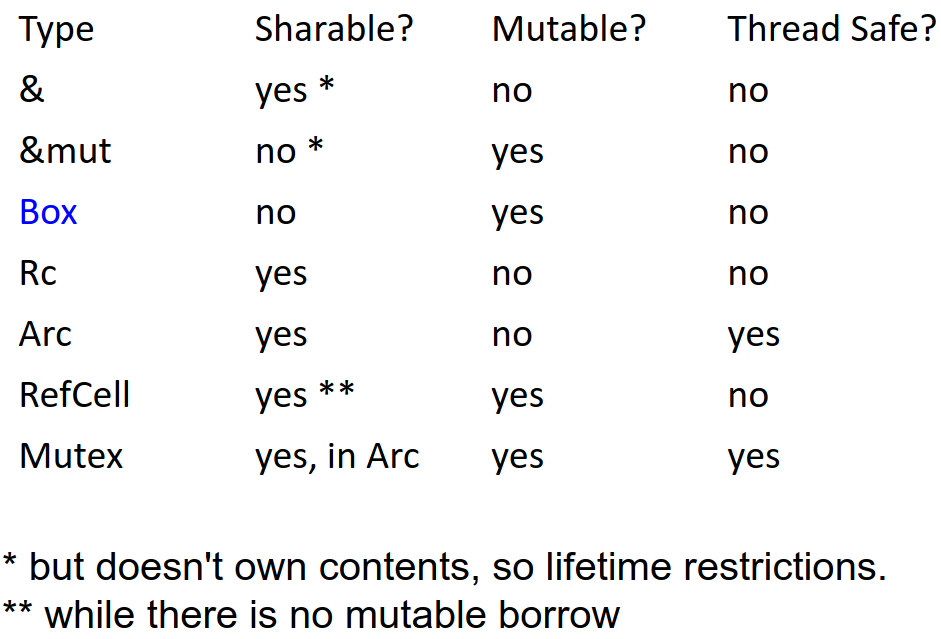
\includegraphics{images/smartpointers.png}
   \caption{Pointers comparison}
   \label{fig:smartpointers}
\end{figure}

\newpage
\section{Functional elements}

\textbf{Closures} can capture non-local variables in three ways,
corresponding to ownership, mutable and immutable
borrowing; 
this is reflected in the trait they implement: \lstinline|FnOnce|,
\lstinline|FnMut| and \lstinline|Fn|.
The trait implemented is inferred.
With \lstinline|move| before \lstinline{||} \lstinline|FnOnce| is enforced.
\begin{lstlisting}
   let x = 5;
   let greater_than_x = |y| y > x; // Parameters within ||
   println!("{}",greater_than_x(3)); // prints "false"
   
   let vector = vec![1, 2, 3, 4, 5]; // stream-like
   vector.iter()
      .map(|x| x + 1)
      .filter(|x| x % 2 == 0)
      .for_each(|x| println!("{}", x));
\end{lstlisting}

\newpage
\subsection{Race conditions}
\begin{paracol}{2}
   \colfill
\begin{lstlisting}[caption={Broken Rust code},label={lst:rust_broken}]
// Rust: does not compile
fn main() {
   let mut counter = 0;
   let task = || {
     // closure
     for _ in 0..100000 {
      counter += 1;
     }
   };
   let thread1 = thread::spawn(task);
   let thread2 = thread::spawn(task);
   thread1.join().unwrap();
   thread2.join().unwrap();
   println!("{}", counter);
}   
\end{lstlisting}

Looking at Listing \ref{lst:rust_arcmutex} on the right:\ns
\begin{itemize}
   \item \lstinline|Arc| is used to share ownership of the Mutex across multiple threads. It ensures that the \lstinline|Mutex| is not deallocated while it is still in use
   
   \item \lstinline|Mutex| ensures that only one thread can access the counter at a time, preventing data races.
   
   \item \lstinline|counter.lock().unwrap()| locks the \lstinline|Mutex| to gain mutable access to the counter. The \lstinline|unwrap()| is used to handle the possibility of the lock being poisoned by a panic in another thread.
\end{itemize}
   \colfill
   \switchcolumn

\begin{lstlisting}[caption={Fixed code with \lstinline|Arc<Mutex<T>>| and \lstinline|move|, but some code duplication is present},label={lst:rust_arcmutex}]
use std::sync::{Arc, Mutex};
use std::thread;

fn main() {
   let counter = Arc::new(Mutex::new(0));
   let counter1 = Arc::clone(&counter);
   let counter2 = Arc::clone(&counter);

   let task1 = move || {
     for _ in 0..100000 {
      let mut num = counter1.lock().unwrap();
      *num += 1;
     }
   };

   let task2 = move || {
     for _ in 0..100000 {
      

      let mut num = counter2.lock().unwrap();
      *num += 1;
     }
   };

   let thread1 = thread::spawn(task1);
   let thread2 = thread::spawn(task2);

   thread1.join().unwrap();
   thread2.join().unwrap();

   println!("{}", *counter.lock().unwrap());
}   
\end{lstlisting}

\end{paracol}

\begin{paracol}{2}
\colfill
Listing \ref{lst:rust_broken} does not compile because Rust does not allow shared mutable state between threads. 
   The closure \lstinline|task| tries to capture \lstinline|counter| by mutable reference because it needs to increment it, but Rust notices it may outlive the borrowed value \lstinline|counter|, so it does not compile.
   
   Rust’s borrowing rules prevent multiple mutable references to the same data at the same time. When you try to spawn two threads with the same closure, both threads would need mutable access to \lstinline|counter|, which is not allowed.
   
   Rust prevents this bug by forcing us to make our intentions explicit. We can fix this by using the \lstinline|Arc<Mutex<T>>|, along with the \lstinline|move| keyword to move the ownership of the closure to the thread.

   Notice that using only \lstinline|move| to move the ownership of the closure to the thread is not enough, because the closure still captures \lstinline|counter| by mutable reference. We need to use \lstinline|Arc<Mutex<T>>| to fix this issue, as in Listing \ref{lst:rust_arcmutex}.
\colfill
   \switchcolumn

   \begin{lstlisting}[caption={Same as Lst.\ref{lst:rust_arcmutex}, but with a function to spawn tasks, avoiding code duplication},label={lst:rust_arcmutex_spawn}]
use std::sync::{Arc, Mutex};
use std::thread;

fn spawn_task(counter: Arc<Mutex<i32>>) -> thread::JoinHandle<()> {
    thread::spawn(move || {
        for _ in 0..100_000 {
            let mut num = counter.lock().unwrap();
            *num += 1;
        }
    })
}

fn main() {
    let counter = Arc::new(Mutex::new(0));
    
    let thread1 = spawn_task(Arc::clone(&counter));
    let thread2 = spawn_task(Arc::clone(&counter));
    
    thread1.join().unwrap();
    thread2.join().unwrap();

    println!("{}", *counter.lock().unwrap());
}
   \end{lstlisting}
   
\end{paracol}



\subsection{\texttt{Sync} and \texttt{Send}}
\lstinline|Send| and \lstinline|Sync| are two strongly related traits regarding multithreading: 
an error is signaled by the compiler if the ownership of
a value \textit{not} implementing \lstinline|Send| is passed to another thread;
for a value to be referenced by multiple threads, it has to
implement \lstinline|Sync|.
\begin{equation}
   \texttt{T} \textit{ implements } \texttt{Send} \Leftrightarrow \texttt{\&T} \textit{ implements } \texttt{Sync}
\end{equation}
\labelitemize{
   Examples
}{
   \begin{itemize}
      \item \lstinline|Arc<T>| is the thread-safe version of \lstinline|Rc<T>| which implements Send and Sync
      \item \lstinline|Mutex<T>| supports mutual exclusive access to a value via a
      lock. It is both Send and Sync, and typically wrapped in Arc
   \end{itemize}
}

\subsection{Unsafety}
Mutable sharing is \textit{inevitable} in the real world, and Rust provides a way to handle it through \textbf{unsafe blocks}.

Rust does \textbf{not} check the memory safety of most operations with raw pointers, they should be encapsulated in a \lstinline|unsafe{}| synctatic structure.
\begin{lstlisting}
   struct Node {
      prev: option<Box<Node>>,
      //next: option<Box<Node>>,
      next: *mut Node // raw pointer
   }
\end{lstlisting}

\begin{lstlisting}
   let a = 3;
   unsafe {
      let b = &a as *const i32 as *mut i32; \\ "I know what I'm doing"
      *b = 4;
   }
   println!("a = {}", a); // prints "a = 4"
\end{lstlisting}

All \textit{foreign} functions are \textit{unsafe} because Rust cannot guarantee their safety.

\begin{lstlisting}
   extern {
      fn write(fd: i32, data: *const u8, len: u32) -> i32;
   }
   fn main() {
      let msg = "Hello, world!\n";
      unsafe {
         write(1, &msg[0], msg.len());
      }
   }
\end{lstlisting}